\section{Appendix}
% ****************

\subsection{Plotting with \texttt{matplotlib.pyplot}}
% ===================================================

The documentation of \texttt{matplotlib} and its modules is quite extensive
but it doesn't give a simple overview of how graphics are organized. Therefore this
section outlines the idea behind \texttt{pyplot} graphics and its components. 

\cmd{pyplot} is a layer on \texttt{matplotlib} to provide graphic facilities
similar to Matlab. \texttt{pyplot} appears to be the preferred way to plot
graphics in \texttt{python/matplotlib}. See also \href{http://matplotlib.org/faq/usage_faq.html}{matplotlib usage} and 
the tutorial \href{https://github.com/ericliang/matplotlib/blob/master/trunk/scipy06/oo_resources/leftwich_tut.txt}
{Getting Started With Matplotlib}.

So, first import the \cmd{pyplot} module:

\begin{verbatim}
import matplotlib.pyplot as plt
\end{verbatim}

and get some dummy data to play with:

\begin{verbatim}
import numpy as np

x= np.array([1, 2, 3, 4])
y= x**2
\end{verbatim}

Here \texttt{x} and \texttt{y} are numpy arrays, although \texttt{pyplot} accepts
any iterable.

\subsubsection{Figure}
% --------------------------
\begin{verbatim}
fig= plt.figure()
\end{verbatim}

\cmd{matplotlib.figure.Figure()} is the top level of a graphics where everything starts
and it is therefore the equivalent of a blank sheet of paper where you draw the plot on. Use \texttt{figure}
to set among other things the \textbf{size} of the figure (in inches) and the \textbf{dpi} resolution,
if applicable. More or less the call \texttt{fig= plt.figure()} is equivalent to
\texttt{R}'s \texttt{g<- ggplot()}. \texttt{figure()} can be called with only default parameters;
in fact, a call to \texttt{Figure} can be skipped altogheter (see below). 

\subsubsection{Axis}
% ------------------

\begin{verbatim}
axes= fig.add_subplot(1, 3, 2)
\end{verbatim}

To draw on a \texttt{Figure} object you need to put a set of \cmd{Axes} where you actually
draw stuff.

\texttt{Axes} can be put with \cmd{.add\_subplot} or \cmd{.add\_axes}. \texttt{add\_subplot}
is similar to \texttt{R} \texttt{par(mfrow= c(n, m))} in that it divides the figure
in \emph{n} rows and \emph{m} columns. The third argument in \texttt{add\_subplot} states
which subplot should be drawn upon. \emph{E.g.} \texttt{fig.add\_subplot(1, 3, 2)}
sets one row, three columns, and draws in the middle subplot (number 2).

Alternatively \cmd{.add\_axes} can be used to specify the characteristics of the
plotting box. It's roughly equivalent to \texttt{R} \texttt{par(mar= c(a, b, c, d))}
in that you set the position of the axes relative to the overall figure. It can also
be used to add plot on top of each other, like figure insets.

The \cmd{Axes} object can be used to control graphic parameters like x- and y-limits,
the axis labels and the plot title. It controls more or less what you can control with \texttt{R}'s \texttt{par()}.

As for \texttt{Figure}, you can add a subplot with only default arguments or skip
the call altogether.

\subsubsection{Plotting}
% ----------------------

\begin{verbatim}
axes.plot(x, y)
\end{verbatim}

Drawing is realized by adding stuff to the \texttt{Axes} object, typically by means
of \cmd{plot()} function. Similar to \texttt{R plot()}, with \texttt{plot} you can
set the plotting style (line, point), colour, etc. See \href{http://matplotlib.org/api/pyplot_api.html#matplotlib.pyplot.plot}
{pyplot.plot} for documentation of setting line styles and plotting features.

\subsubsection{Rendering}
% ----------------------

\begin{verbatim}
fig.savefig('filename.pdf')
fig.show()
plt.close()
\end{verbatim}

The actual plot is visualized with the \cmd{show()} method and saved to file with
\cmd{savefig()} method. By default, file format is deduced from file extension.
Finally, call \cmd{close} to close the grahic device(s).

\subsubsection{In practice...}
% ----------------------------

In practice you can take shortcuts to create plots. It is not strictly necessary
to explicitly set up a \texttt{Figure} and \texttt{Axes} object.

\begin{verbatim}
plt.plot(x, y, 'r--', lw= 2)
plt.plot(x, y, 'bo', markersize=12)
plt.xlabel('x-lab')
plt.xlim([0, 5])
plt.rc('font', size= 20)
plt.grid()
plt.savefig('figs/app_simple.pdf', bbox_inches= 'tight')
plt.show()
\end{verbatim}

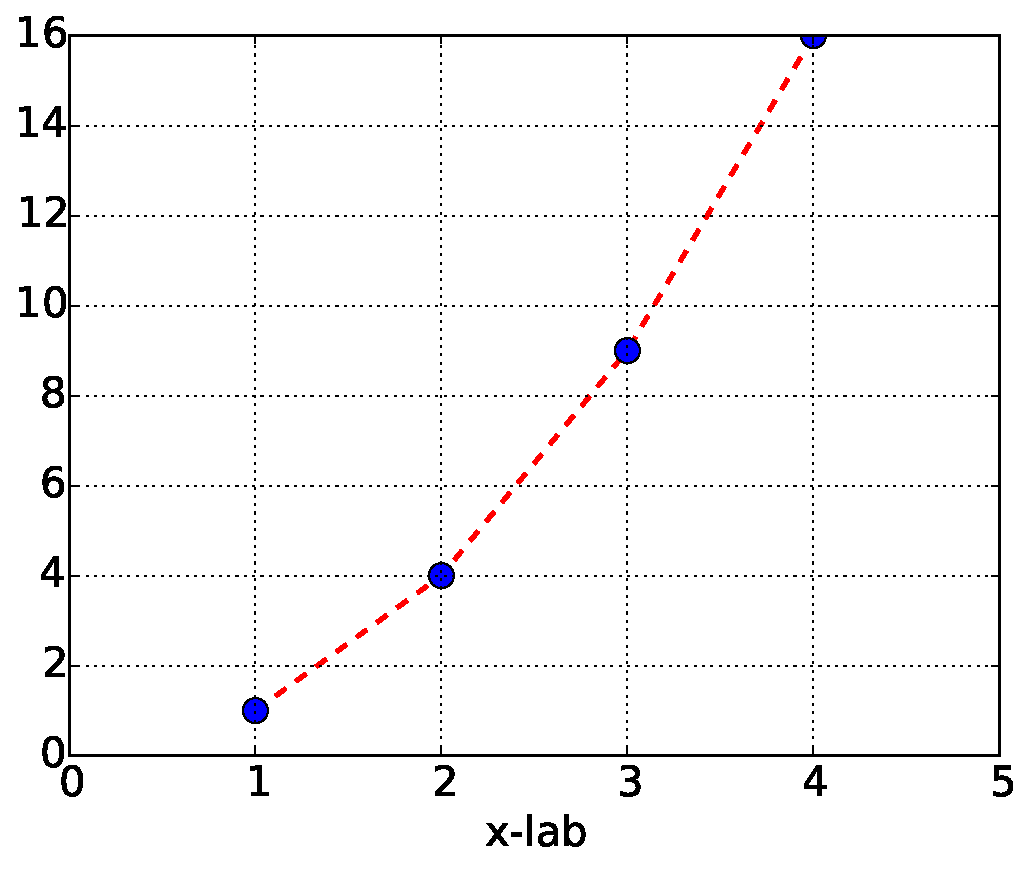
\includegraphics[width=0.5\linewidth]{figs/app_simple.pdf}

For simple plots, you can just call \cmd{plt.plot()} with the data to plot and
optional graphic paramaters. The bare minimum to see an xy-plot is just
\texttt{plt.plot(x, y); plt.show()}

Note that you keep adding features using \texttt{plt.<feature>},
then when you call \texttt{savefig} or \texttt{show} everything comes together.
In contrast to \texttt{R}, the order with which you add these features doesn't
matter. However, if you want to save to file \emph{and} show on screen, remember
to call \texttt{savefig} first and \texttt{show} then.

\begin{verbatim}
plt.rc('font', size= 8)
fig, axlst = plt.subplots(1, 3, sharex=True, sharey= True)
axlst[0].plot(x, y)
axlst[1].plot(x, y*2)
axlst[2].plot(x, y*3)
fig.subplots_adjust(wspace= 0.1)
fig.set_size_inches(18/2.54, 6/2.54)
fig.savefig('figs/app_subplot.pdf')
fig.show()
\end{verbatim}

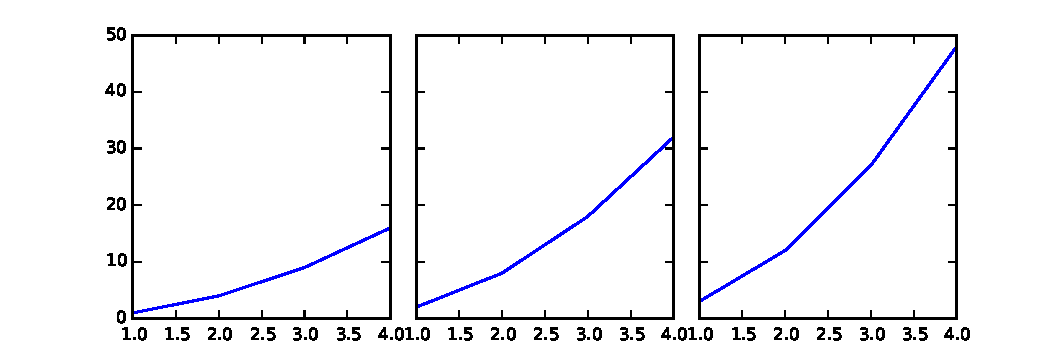
\includegraphics[width=\linewidth]{figs/app_subplot.pdf}

For multiple plots it might be best to set up the \texttt{Figure} object and the
list (array actually) of subplots in one call to \cmd{plt.subplots()}. Each element
of the array contains an \texttt{Axes} object that can be individually populated.
The \texttt{Axes}'s can be juxtaposed by playing with the method \cmd{Figure.subplots\_adjust}.
For example to set the spacing. 

\subsubsection{Example}
% ---------------------

\begin{verbatim}

fig= plt.figure()
ax1= fig.add_subplot(1, 3, 1)
ax1.plot(x, y, 'r--')
ax2= fig.add_subplot(1, 3, 2)
ax2.plot(x, y, 'pg')
ax3= fig.add_subplot(1, 3, 3)
ax3.plot(x, y, 'p')
for i, txt in enumerate(x):
    ax3.annotate(txt, (x[i], y[i]))
fig.show()
\end{verbatim}